\def\year{2018}\relax
%File: formatting-instruction.tex
\documentclass[letterpaper]{article} %DO NOT CHANGE THIS
\usepackage{aaai18}  %Required
\usepackage{times}  %Required
\usepackage{helvet}  %Required
\usepackage{courier}  %Required
\usepackage{url}  %Required
\usepackage{graphicx}  %Required

\usepackage{multirow}
\usepackage{multicol}
\usepackage{array}
\usepackage{graphicx}
\usepackage{footnote}
\usepackage{amsmath, bm}
\usepackage{color}
\usepackage{xcolor}
\usepackage{xspace}

\newcommand{\FIXME}[1]{\textcolor{red}{FIX:}\textcolor{red}{#1}}
\newcommand{\DS}{\texttt{DS}\xspace}
\newcommand{\KB}{\texttt{KB}\xspace}
\newcommand{\red}[1]{\textcolor{red}{#1}}
\newcommand{\brown}[1]{\textcolor{brown}{#1}}
\newcommand{\green}[1]{\textcolor{green}{#1}}
\newcommand{\blue}[1]{\textcolor{blue}{#1}}
\newcommand{\cyan}[1]{\textcolor{cyan}{#1}}

\frenchspacing  %Required
\setlength{\pdfpagewidth}{8.5in}  %Required
\setlength{\pdfpageheight}{11in}  %Required
%PDF Info Is Required:
  \pdfinfo{
/Title (Event Extraction without Human-annotated Text)
/Author (Anonymous AAAI submission)}
\setcounter{secnumdepth}{0}
 \begin{document}
% The file aaai.sty is the style file for AAAI Press 
% proceedings, working notes, and technical reports.
%
\title{Event Extraction without Human-annotated Text}
\author{Anonymous AAAI submission}
\maketitle

% TODO: Merge each section to one file
\begin{abstract}
Supervised learning is an effective method for building event extraction systems. The effectiveness of the learning heavily depends on
the quality of the training datasets. Existing event extractor systems are typically built upon expert-annotated datasets. However, due
to drastic efforts involved in annotating text, these datasets are usually small and cover only a limited variety of event types. This
limits the quality of learned event extractor, making it hard to generalize. In this paper, we investigate ways to generate training
datasets that require little expert involvement but can cover a richer set of event types. We achieve this by employing distant
supervision to automatically create event annotations from unlabelled text using existing structured knowledge bases or tables. We then
develop a novel neural network model with post inference, to detect multi-typed event mentions \FIXME{ZW: reviewers may not know what is
a event mention} with corresponding arguments. Experiments on the datasets collected through Freebase and Wikipedia tables show that it
is possible to learn to extract events of rich types without human-annotated training data. \FIXME{ZW: Will come back to the experimental
results later.}

%Existing event extraction systems are typically investigated in a supervised learning paradigm, which heavily relies on the quality of
%expert-annotated datasets. Due to the drastic efforts involved in text annotation, the human-annotated datasets are typically small, only
%covering a limited variety of event types. This limits This limits the quality of learned event extractor, making it hard to generalize.


%In this paper, we address the problem of automatically building event extractors for rich event types with little expert involvement. We
%achieve this by employing distant supervision to automatically create event annotations from unlabelled text using structured knowledge
%bases or tables. We propose a novel neural network model with post inference, to detect multi-typed event mentions with corresponding
%arguments.
%% We evaluate our approach by investigating the feasibility of  automatically collecting training data for event extraction from both
%Experiments on the datasets collected through Freebase and Wikipedia tables show
%that
%%our proposed extraction model is designed to identify both typed event mentions and typed arguments.
%% Both automatic and manual evaluations demonstrate that
%it is possible to learn to extract events of rich types without human-annotated training data.

%
%and rely on expert-annotated datasets, with limited event types.
%%such as ACE and ERE event extraction frameworks.
%However, designing and constructing these
%high-quality corpora, usually with limited size and coverage of event types,  is costly, which
%makes learned extractors hard to generalize.  With the essence of distant supervision,
%%Inspired by some Freebase schemas which share similar structures with ACE event templates,
%we investigate the possibilities of automatic construction of training data for various event types
%with the help of structured knowledge bases.
%the following problems in this paper: can we generate a feasible dataset for event extraction with Freebase automatically and is it possible to extract events on this dataset.
%We first propose four hypotheses based on our observation and produce our dataset accordingly. Then,
%We further propose a novel neural network with ILP-based post inference, committing to
%handling two challenges in event extraction: multi-type events and multi-word arguments.
%Both automatic and manual evaluations demonstrate that it is possible to learn to extract various  events, according to existing knowledge bases, without human-annotated training data.
\end{abstract}

\section{Introduction}
%Automatically extracting events from natural text remains a challenging task in information extraction. Among diverse types of event extraction systems, the extraction task proposed by Automatic Content Extraction (ACE) \cite{doddington2004automatic} is the most popular framework, which defines two main terminologies: \textbf{trigger} and \textbf{argument}. The former is the word that most clearly expresses the occurrence of an event. The latter is a phrase that serves as a participant or attribute with a specific role in an event.
%
%However, constructing training data for ACE task is expensive. First, linguists are required to summarize a large amount of text to elaborately design templates about potential arguments for each event type. Second, rules should be explicitly stated to guide annotators. In spite of detailed guidelines, there is still disagreement among human annotators about what should (not) be regarded as triggers/arguments.
%For example, can a prepositional phrase or a portion of a word trigger an event, e.g., \textit{in prison} triggers an \emph{arrest} event,
%or, \textit{ex} in \textit{ex-husband} triggers a \emph{divorce} event?
%Besides, ACE event extraction systems have two major limitations:   single-token trigger labeling, and one type for one event.

Event extraction is a key enabling technique for many natural language processing (NLP) tasks. The goal of event extraction is to detect,
from the text, the occurrence of events with specific types, and to extract arguments (i.e. typed participants or attributes) that are
associated with an event. Current event extractor systems are typically built through applying supervised learning to learn over labelled
datasets. This means that the performance of the learned model is bound by the quality and coverage of the training datasets.

To generate training data for event extraction, existing approaches all require manually identifying -- if an event occurs and of what type
-- by examining the event trigger\footnote{In the event extraction task, a trigger is the word or phrase that most clearly expresses the
occurrence of an event. For example, \textit{ex} in \textit{ex-husband} may trigger a \emph{divorce} event.} and arguments from each
individual training instance. This process requires the involvement of linguists to design annotation templates and rules for a set of
predefined event types, and the employment of annotators to manually label if an individual instance belongs to a predefined event type.


To determine an event type, existing approaches  all require \emph{explicitly} identifying the event trigger from the text to associate the
text with an event. Because identifying event triggers is non-trivial~\FIXME{\cite{}}, human involvement is deemed necessary. However, this
thus makes the quality and the number of the generated instances directly dependent on the skill and available time of the
annotators~\cite{aguilar2014comparison,song2015light}. To scale up event extractor training, we therefore must take human annotators out
from the loop of data labeling.


This work develops a novel approach to automatically label training instances for event extraction. Our key insight was that while event
triggers are useful, they do not have to be explicitly captured. Structured knowledge bases (\KBs) such as Freebase already provide rich
information of arguments, which is organized as structured tables,  to enable us to automatically infer the event type without explicitly
knowing the trigger. For example, an \emph{marriage} event does not always have to be identified through finding the \emph{married}
trigger, as a \emph{spouse} argument also implies
such an event. %In this paper, we show that structured tables in some knowledge bases already imply the occurrence of certain events.


If we can find ways to exploit structured tables or lists, a single entry can then be used to label a large number instances without the
involvement of human annotators. Such an approach is known as distant supervision (\DS). Recent
studies~\cite{mintz2009distant,zeng2015distant} have demonstrated its effectiveness in various NLP tasks. The central idea of of \DS is to
use the knowledge extracted from a known knowledge base to \emph{distantly supervise} the process of training data generation using another
dataset. By employing \DS, our approach is able to produce a large number of high-quality training instances.

Under this new \DS paradigm, we develop a novel event extractor architecture based on neural networks and linear integer programming. One
of the key innovations of our approach is that the model does not rely on explicit trigger information. Instead, it uses a set of key
arguments to characterize an event type. As a result, it eliminates the need to explicitly identify the event trigger, a process that
requires heavy human involvement.

We evaluate our approach by  applying it to perform sentence-level event extraction. To generate training data, we use Freebase to
automatically label texts from a subset of Wikipedia articles. We then learn an event extractor using the generated data and use the
learned model to extract events from unseen Wikipedia articles.

Using \FIXME{24} structured tables from Freebase, we are able to generate over 100 thousands training instances within two hours. This
results in a training dataset that is 100x greater than the widely used ACE dataset -- which took \FIXME{xx man-months} to
build\FIXME{~\cite{}}. We show that the quality of the automatically generated dataset is comparable to ones that were manually constructed
by human experts. Experimental results show that our new approach of data generation and modeling not only allows building a more efficient
event extractor, but also enables multi-typed event detection -- a feature that none of the existing event extractors offers -- but is much
needed.



%The aforementioned drawbacks of ACE event extraction systems motivate us to
%It would be interesting to see (1) can we automatically build a dataset for event extraction without experts involved?
%and (2) can we have an event extractor that handles more realistic scenarios, e.g.,  when trigger annotations are unavailable, or events with more than one type.


%This paper presents a novel approach for automatic training data generation, specifically targeting event extraction. Our approach advances prior work in two aspects: (1) it does not rely on expert-annotated texts (hence it reduces expert involvement)
%and (2) supports multi-typed event extraction. The former is achieved by automatically collecting training data through indirect supervision from structured knowledge bases or knowledge tables to automatically label event structures from plain text. The later is achieved by proposing a novel neural network model with post inference to detect multi-typed events without relying on explicit trigger annotations.

%Our first insight is that structured knowledge bases (\KB) typically organize
%complex structured information in tables; and such knowledge tables often share similar structures with ACE event definitions, i.e., a particular entry of such tables usually implies the occurrence of certain events.
%Recent studies \cite{mintz2009distant,zeng2015distant} have demonstrated the effectiveness of \KB as distant supervision (\DS) for binary relation extraction. In this paper, we aim to extend \DS to extract events of n-ary relations and multiple arguments (rather than just binary
%relation). One of the hurdles for doing this is the lacking of explicit trigger information in existing \KB.
%Our solution is to use a group of \textbf{key arguments} rather than explicit triggers to capture a particular event. For example, we can use \emph{spouse} as the key argument to identify \emph{marriage} events.


%However, there are two major challenges when leveraging KB to event extraction: first, event structures are more complex than binary relations. They can be represented as $\langle event\_type, argument_1, \ldots, argument_n\rangle$, which are n-ary relations with various numbers of arguments. Second, there is no explicit trigger information in any existing knowledge base.
%However, we find that for a particular event type, there is a group of \textbf{key arguments} which together can imply an event instead of explicit triggers. For example, ``\emph{spouse}'' is the key argument of ``\emph{marriage}'' events, while ``\emph{location of ceremony}'' is too generic to become a key argument. Therefore, we put forward a distant supervision approach to event extraction: a sentence that contains all key arguments of an event is likely to express that event in some way. To explore the sets of key arguments, we investigate different hypotheses for better data quality and quantity.

% Therefore, to explore the distant supervision (\texttt{DS}) assumption in event extraction, we investigate different hypotheses for better data quality and quantity. Among them, the vital one is that, for a particular event type, there is a group of \textbf{key arguments} which together can imply an event instead of explicit triggers.


%We utilize Freebase as our knowledge base and Wikipedia articles as text for data generation as a major source of Freebase is the tabular data from Wikipedia \cite{mintz2009distant}.
% According to Mintz et al. \shortcite{mintz2009distant}, because a major source of Freebase is the tabular data from Wikipedia, making it a natural fit with Freebase.
%Figure~\ref{fig:3} illustrates examples of sentences annotated by our algorithm.

%Our second innovation is that unlike previous studies which focus on tasks defined by the ACE evaluation framework
%\cite{ahn2006stages,li2013joint,chen2015event,nguyen2016joint}, we propose a novel event extraction paradigm with key arguments to
%characterize an event type. We consider event extraction as two sequence labeling subtasks, namely event detection and argument detection.
%Inspired by neural network models in sequence labeling tasks \cite{huang2015bidirectional,lample2016neural}, we utilize BLSTM-CRF models to
%label key arguments and non-key arguments in each sentence separately. However, event structures are not simple sequences and there are
%strong dependencies among key arguments. We therefore reformulate the hypotheses as constraints, and apply linear integer programming to
%output multiple optimal label sequences to capture multi-typed events.

%We evaluate our approach by applying it to automatically collect training data with both Freebase and Wikipedia tables.
%Our proposed event extractor is used to identify typed event mentions with typed roles. Our experimental
%results on both automatic and
%manual evaluations show that our approach can effectively extract a rich types of events without expert-annotated training data. %\FIXME{quantified numbers?}

%In this paper, we exploit existing structured knowledge bases, e.g., Freebase, as distant supervision to automatically annotate event structures from plain text without human annotations. We further propose a novel event extraction paradigm that harnesses key arguments to imply certain event types without explicit trigger annotations. We present an BLSTM-CRF model with post inference to extract both Freebase-style events as well as multi-type event mentions on the generated dataset, which is demonstrated effective by both manual and automatic evaluations.

\section{Motivation}
\begin{figure}
  \centering
   \subfloat[][An example sentence from Wiki text]{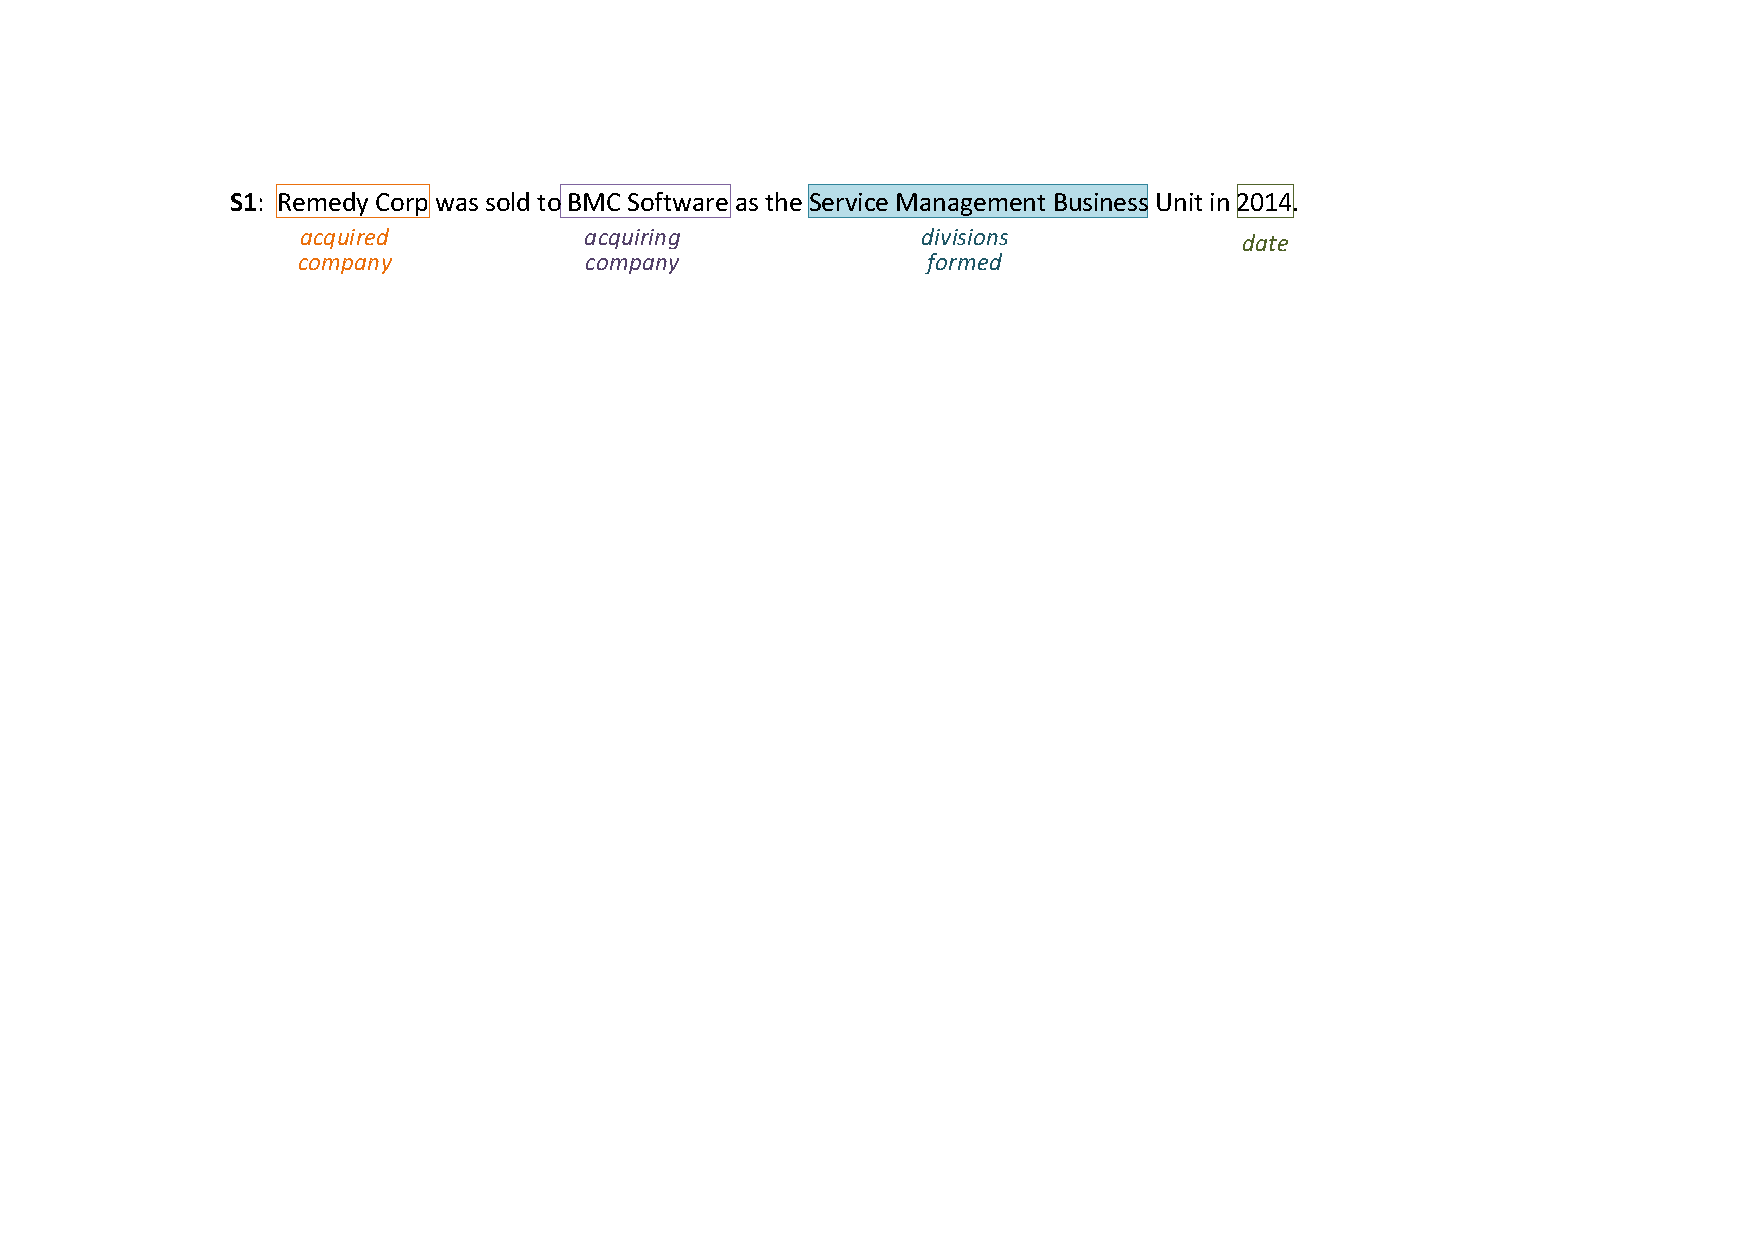
\includegraphics[width=0.5\textwidth]{figs/example.pdf}}
   \\
   \subfloat[][ Entry of \texttt{business.acquisition} in Freebase]{
        \scriptsize
        \begin{tabular}{llllp{1.6cm}}
        \toprule
        id & company\_acquired & acquiring\_company & date & divisions\_formed\\
        \midrule
        m.07bh4j7 & Remedy Corp & BMC Software & 2004 & Service Management Business Unit\\
        \bottomrule
        \end{tabular}

   }
  \caption{The event type of the sentence shown in (a) can be automatically inferred using the structured table given by Freebase in (b).}
  \label{fig:example}
\end{figure}


%The task of event extraction is to (1) detect the occurrence of events with specific types and (2) extract arguments (i.e. typed
%participants or attributes) that are associated with an event.
As a motivation example, consider a sentence extracted from a Wikipedia article, shown in Figure~\ref{fig:example} (a). To detect the event
type, traditional approaches require identifying the trigger, \emph{sold}, and associating it with an event type -- a business acquisition
event in this case.


For this particular sentence, identifying the trigger is not necessary for determining the event type. Figure~\ref{fig:example} (b) shows a
Compound Value Type (\CVT) entry from Freebase (\FB)~\cite{bollacker2008freebase}. Here, a \CVT organizes complex structured data with
multiple \emph{properties} in a table\footnote{Therefore, we also use the term ``argument" to refer to a \CVT property for the rest of the
paper.}. Using this \CVT schema, one can easily map the three arguments of sentence S1, \emph{Remedy Corp}, \emph{BMC Software}, and
\emph{2004}, respectively to their prosperities, \texttt{company\_acquired}, \texttt{acquiring\_company}, and \texttt{date}. Here each
property essentially describes the role of an argument in the sentence; and in combination, all arguments define a
\texttt{business.acquisition} event.

This example shows that \CVT information can be used to infer event type without explicit trigger information. If we can utilize such \CVT
information, we can then label sentences without needing to explicitly identifying the trigger. As a result, we can free annotators from
the labour-intensive manual process. In this work, we develop a simple, yet effective technique to automatically generate training data by
exploiting the prior \CVT knowledge.

A natural question to ask is that ``How useful are \CVT-like structured information?". Later in this paper, we show that structured
knowledge base, tables or lists that are used to sum up certain activities can be a useful source of supervision data generation for event
extraction -- using 24 \CVTs, we managed to automatically generate 100 thousands instances from a subset of the Wikipedia articles.

%
%This work develops a simple, yet effective technique to automatically generate training data by exploiting the prior \CVT knowledge from
%%various datasets, including \FB and Wikiedia pages. Our work shows that it is possible to scale up training data generation for event
%%extraction with little human involvement.
%In the next section, we describe g our approach of automatic traning data generation in more
%details.


%%
%%Instead of asking human annotators to manually tag each individual training sentence, we use a predefine structure table to automatically
%%identify event types. In this way, experts are only required to construct a table of event types and arguments associated with each type;
%%our method can then use the table to automatically label many sentences that contains these arguments. By doing so, we essentially reduce
%%human involvement as now experts now only need to construct a table with a small number entries. \FIXME{zw: some of these need to go to
%%introduction.}  In this work, we find that structured  knowledge bases (\KB) already provide a structure table which can be used to
%%accurately infer the occurrence of certain types in real-world text.
%
%
%
%%
%%\section{The Event Extraction Task}
%%%\subsection{Event Definition}
%%% 给出相关术语的定义,subsection名字起得对吗?
%%Event extraction aims to detect the occurrence of events with specific types and extract their typed participants or attributes from text. We clarify the following terminologies within our work:
%%\begin{itemize}
%%	\item \textbf{Event mention}: a phrase or sentence within which an event is described, including its type and arguments.
%%	\item \textbf{Argument}: an entity mention, temporal expression or value that is involved in an event, with specific roles.
%%	\item \textbf{Key argument}: the argument that plays an important role in one event, and helps to distinguish with other events. % 要不要举例说明什么是key argument?这里再举例会不会和introduction里面的举例重复?
%%	% 没有地方的时候,argument role可以删掉(我看别人ACE定义的时候都讲了这个就先放上来了)
%%	%\item \textbf{Argument role}: the relationship between an event and its involved argument.
%%\end{itemize}
%
%\subsection{Indirect Supervision for Event}%{Tabular Data}
%% 缺一句连接的话?
%We first utilize Freebase~\cite{bollacker2008freebase} as a source of supervision to guide our data construction, %the structured knowledge base.
%% and there are three basics concepts: \emph{instance}, \emph{type} and \emph{property}. \emph{Instances} are entries in Freebase. \emph{Types} are different perspectives of \emph{instances}.
%where \textbf{\emph{Compound Value Type}} (CVT) is a special type to represent complex structured data % where entries are described
%with multiple \emph{properties}, usually organized in a table. Some CVT schemas indeed imply certain events, e.g., \emph{business.acquisition},
%% \emph{military.military\_service} and \emph{people.marriage},
%and closely resemble to event structures, where CVT properties can be treated as event arguments\footnote{
%Therefore, we also use the term ``argument'' to refer to CVT property in the rest of paper.}. % 直接在这里说CVT property其实就是argument,后面描述的时候不会太咯嗦
%As shown in Figure~\ref{fig:3}, the properties of CVT \emph{business.acquisition} actually can be used to label arguments of the events mentioned in S1 and S2.
%We use the Freebase copy of 2013-06,  %version of Berant et al. \shortcite{berant2013semantic},
%containing 1010 CVTs. After manually filtering out those % CVTs that
%describing Freebase structure or irrelevant to events, %(e.g., \emph{food.recipe\_ingredient})
% we obtain 24 CVTs with around 280 million instances.
%
%\begin{figure}[h]
%	\centering
%	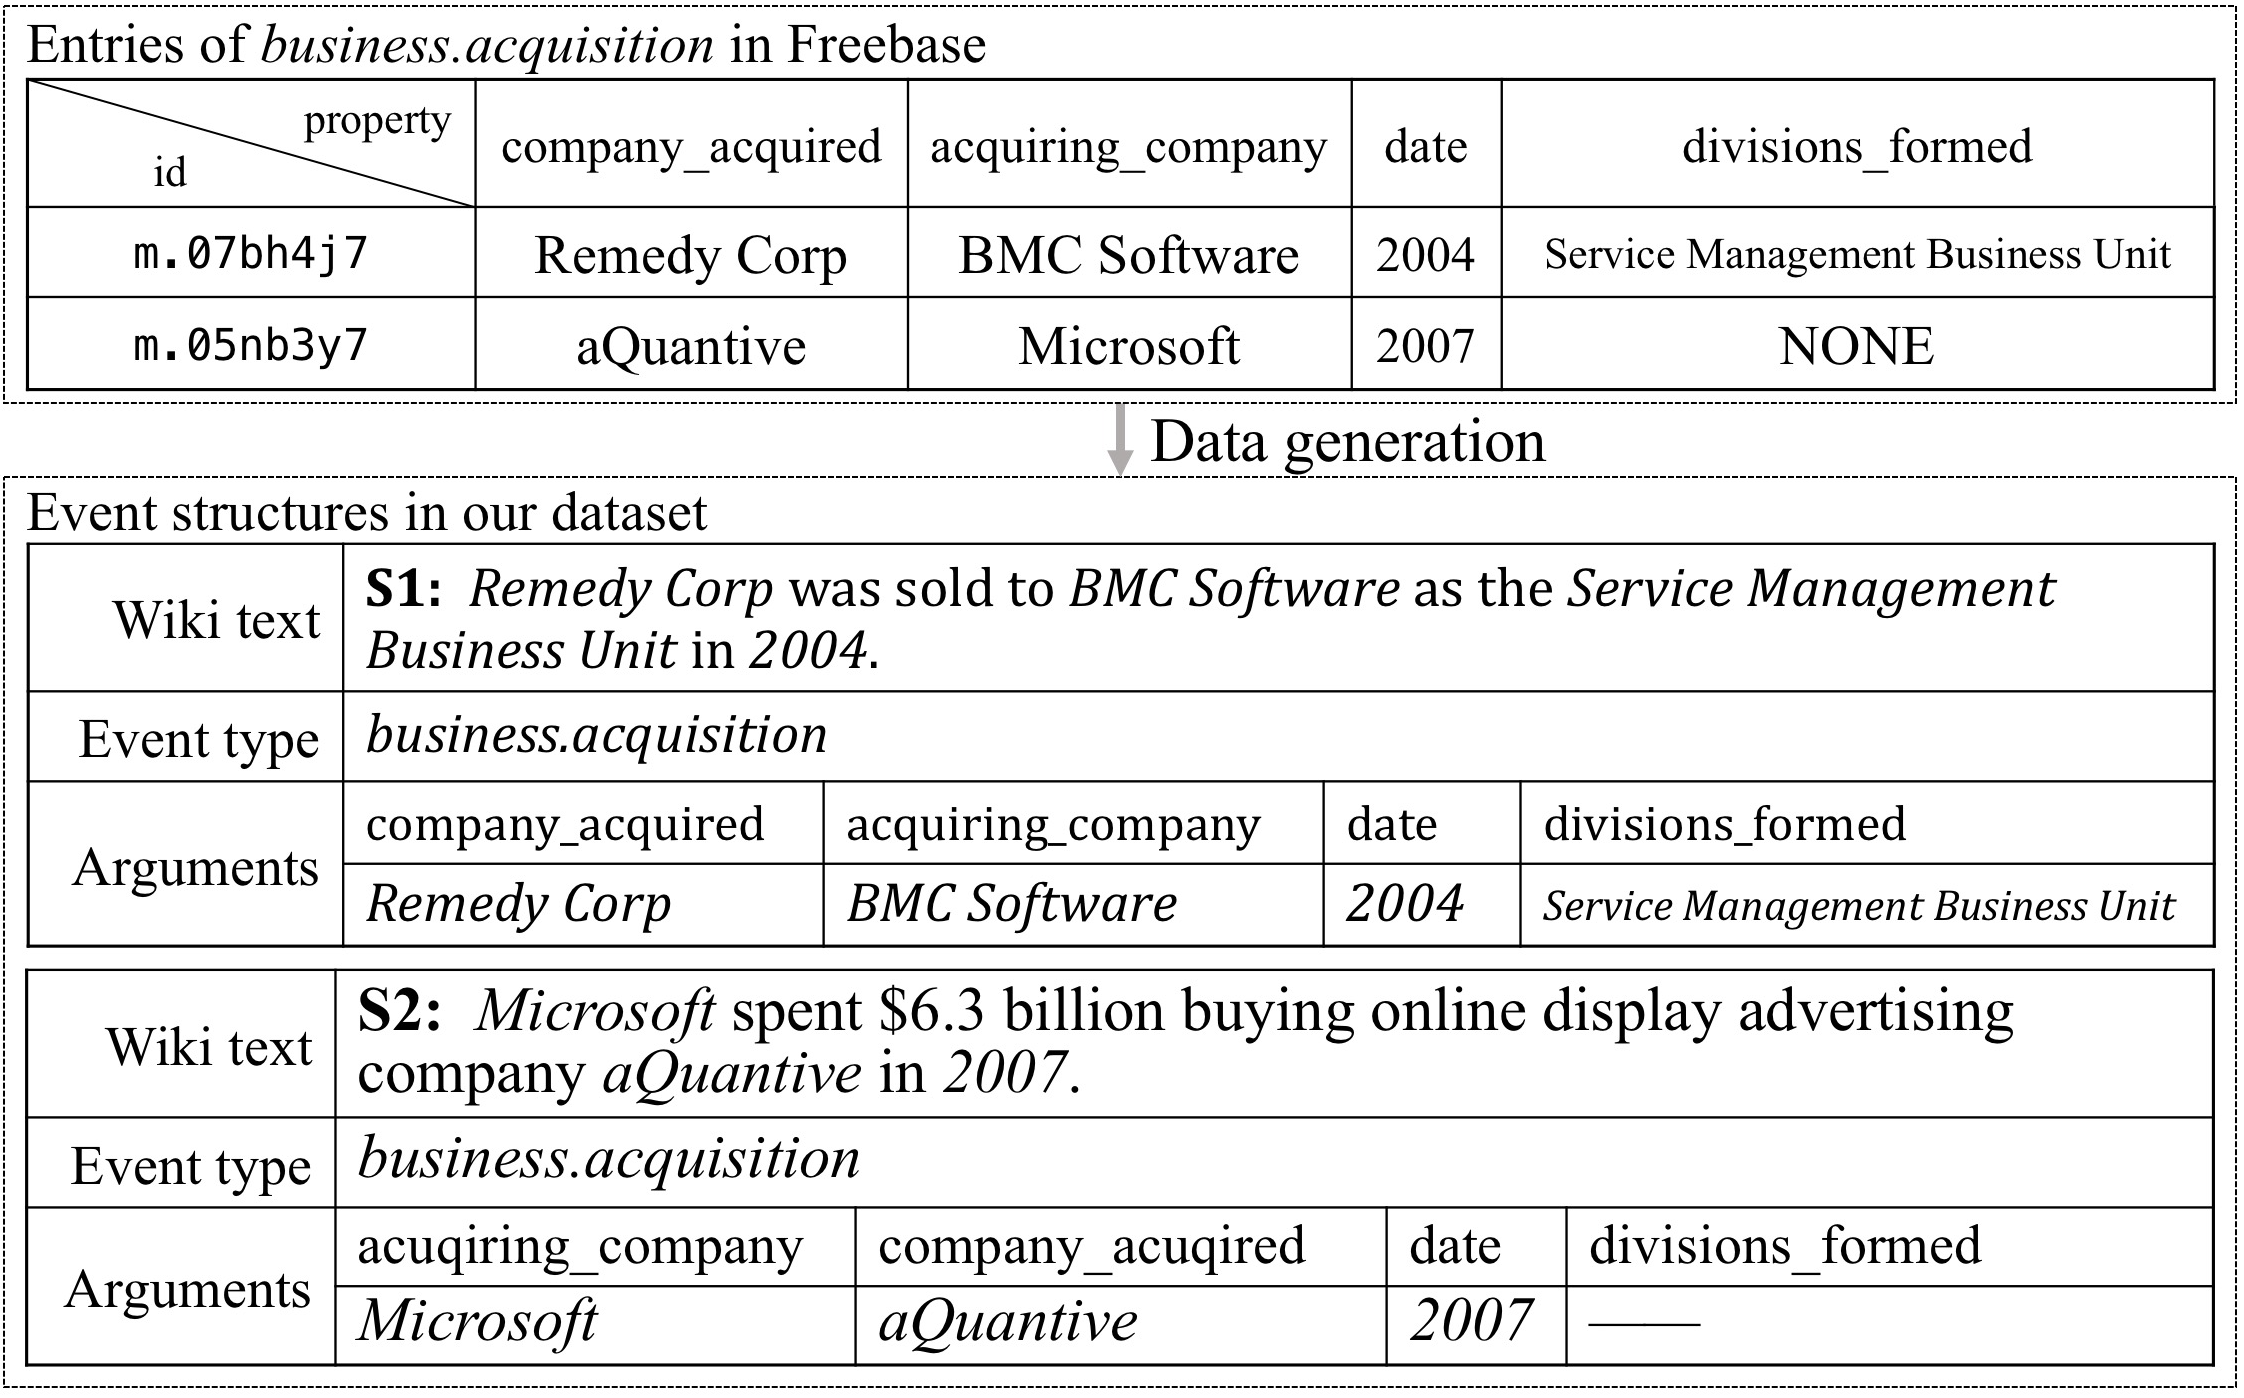
\includegraphics[width=.48\textwidth]{figure1.png}
%	\caption{Examples of a CVT table in Freebase, and labeled sentences in our dataset. \emph{Company\_acquired}, \emph{acquiring\_company} and \emph{date} are key arguments in \emph{business.acquisition}. \label{fig:3}}
%\end{figure}
%%
%Besides structured knowledge base, tables or lists that are used to sum up certain activities or occasions could be considered as a source of supervision for event extraction, as well.
%We thus investigate tables collected from Wikipedia pages, potentially referring to three types: winning of the Olympics, music and film awards, mergers and acquisitions\footnote{For example, \url{https://en.wikipedia.org/wiki/List_of_mergers_and_acquisitions_by_IBM}}.



%\subsection{Dataset Construction\label{datagen}}
%% 在哪里说其实 property 在后面就是 argument 了
%Here, we employ the event-related entries of Freebase CVT tables to illustrate how to automatically annotate event mentions in Wikipedia's articles, with the essence of distant supervision (\textbf{\texttt{DS}}): \textit{A sentence that contains \textbf{all key arguments} of an entry in an event table (e.g., CVT table) is likely to express that event}.
%%\begin{quote}
%%	\textbf{\texttt{DS}}: A sentence that contains all key arguments of an entry in an event table (e.g., CVT table) is likely to express that event in some way.
%%\end{quote}
%We will then label this sentence as a mention of this CVT event, and the words or phrases that match this entry's properties as the involved arguments, with the roles specified by their corresponding property names.
%
%We regard a sentence as \emph{positive} when it mentions the occurrence of an event, or  \emph{negative} otherwise.
%For example, S1 and S2 are positive examples with their arguments in italics and underlined (also shown in Figure~\ref{fig:3}), while S3 and S4 are negative.
%%
%\begin{quote}
%	\textbf{S1}: \underline{\emph{Remedy Corp}} was sold to \underline{\emph{BMC Software}} as the \underline{\emph{Service}} \underline{\emph{Management Business Unit}} in \underline{\emph{2004}}.
%\end{quote}
%\begin{quote}
%\textbf{S2}: \underline{\emph{Microsoft}} spent \$6.3 billion buying online display advertising company \underline{\emph{aQuantive}} in \underline{\emph{2007}}.
%\end{quote}
%\begin{quote}
%\textbf{S3}: Microsoft hopes aQuantive's Brian McAndrews can outfox Google.
%\end{quote}
%\begin{quote}
%\textbf{S4}: On April 29th, Elizabeth II and Prince Philip witnessed the marriage of Prince William.
%\end{quote}
%
%The selection strategy for key arguments of a given event type is based on two criteria: (1) \emph{Key arguments should have high importance value}; (2) \emph{Key arguments should include time-related arguments}.
%% \paragraph{H1: Positive sentences should contain all properties}
%
%% For example, S1 contains all the properties of instance $m.07bh4j7$ with a CVT type \emph{business.acquisition}, we thus consider S1 as a positive sample implying an event about \emph{business.acquisition}, and \emph{BMC Software}, \emph{Remedy Corp}, \emph{Service Management Business Unit} and \emph{2004} will be labeled as the arguments that play the role of \emph{acquiring\_company}, \emph{company\_acquired}, \emph{divisions\_formed}, and \emph{date} in this event, respectively.
%% However, in practice, we realize that \emph{H1} is too strict that excludes a great many positive sentences like S2.
%% In practice, we find that \emph{H1} is too strict to include many positive sentences like S2.
%% We thus relax \emph{H1} by replacing \textbf{all properties} with \textbf{all key properties}.
%
%The \emph{importance value} of an argument $arg$ (e.g., \emph{date}) to its event type $cvt$ (e.g., \emph{business.acquisition}) can be defined as:
%\begin{equation}
%	I_{cvt, arg} = log \frac{count(cvt, arg)}{count(cvt) \times count(arg)}
%\end{equation}
%where $count(cvt)$ is the number of instances of type $cvt$, $count(arg)$ is the number of times $arg$ appearing in all CVT types, and $count(cvt, arg)$ is the number of $cvt$ instances that contain $arg$.
%
%% We discover that for many CVTs, their key properties do not take into account time property.
%% time-related argument叫得对吗?本来的想说的是,取值为时间的argument
%Although time-related arguments are often missing in the currently imperfect KBs,
%they are indeed crucial to indicate the actual occurrence of an event, e.g., S3, containing \emph{Microsoft} as \emph{acquiring\_company} and \emph{aQuantive} as \emph{company\_acquired} but without time-related arguments, will be mistakenly considered as a positive sample for event \emph{business.acquisition}.
%% while contain all key properties of an instance, resulting in mistaking \emph{Microsoft} for \emph{acquiring\_company}, and \emph{aQuantive} for \emph{company\_acquired}.
%% By adding \emph{date} to the set of key properties, S3 will be filtered.
%
%Intuitively, two arguments involving in the same event mention are likely to be closer within the syntactic structure.
%% , which will help to eliminate negative samples.
%% We thus set the maximum distance between two key arguments as 2 empirically.
%%, i.e., for a candidate sentence, if a pair of key arguments violates this constraint, it is supposed to be negative.
%% Given the dependency parsing tree in Figure~\ref{fig:2}, S4 is negative because the distance between \emph{Prince Philip} and \emph{marriage} is 3.
%
%\begin{figure}
%\centering
%	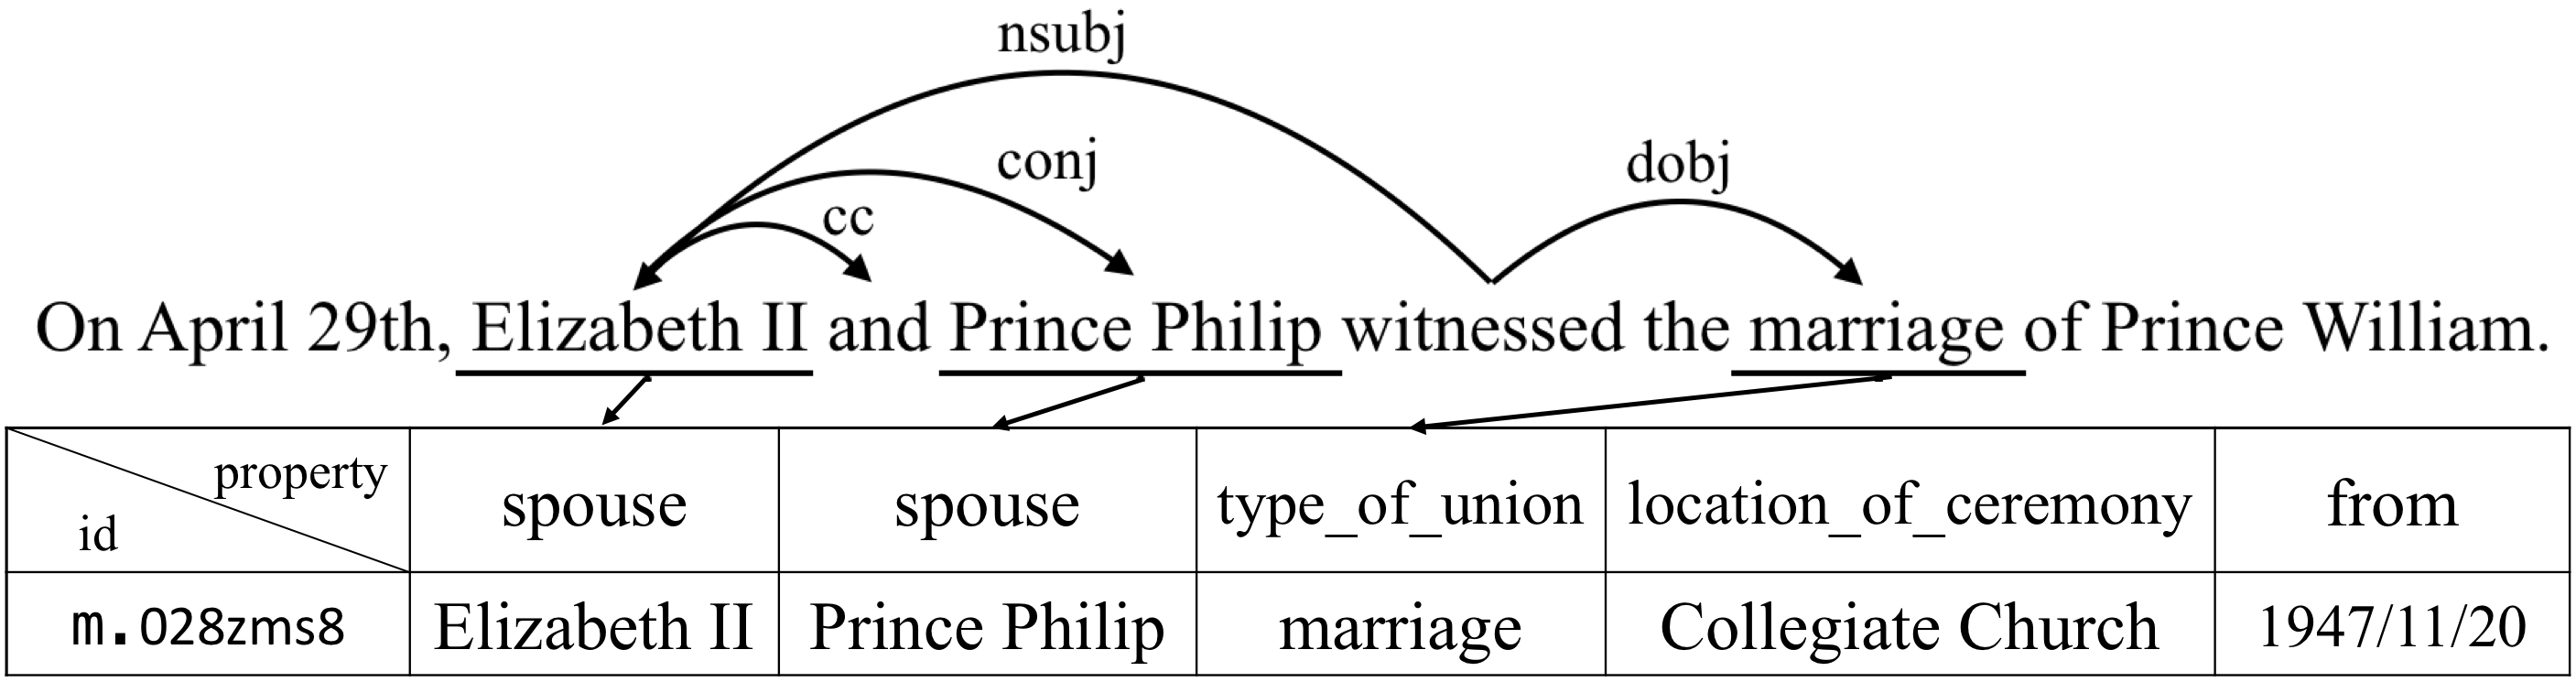
\includegraphics[width=.48\textwidth]{figure2.png}
%	\caption{The dependency tree of S4, which partially matches an entry of \emph{people.marriage}. \label{fig:2}}
%\end{figure}
%
%We conduct a series of manual evaluations on the quantity and quality of the datasets produced by different strategies (see Sec~\ref{sec:evalhypo}), and
%% following strategy produces the best dataset, thus serves as
%our final strategy is:
%for each CVT, we first sort all its arguments in descending order by their importance values, and select the top half arguments as key arguments.
%We then include the time-related argument with highest importance value as a supplementary key argument.
%Finally, we eliminate sentences in which the dependency distances between any two key arguments are greater than 2.

% 好像没地方了,先不写了
% \begin{table}
% \centering
% \small
% \begin{tabular}{|l|l|} \hline
% CVT & Key arguments \\ \hline
% award.award\_honor & award\_winner, award, \ldots, year \\ \hline
% film.performance & actor, film, character \\ \hline
% education.education & institution, student, end\_date \\ \hline
% business.employment\_tenure & company, title, person, from \\ \hline
% \end{tabular}
% \caption{Examples of key arguments of four CVTs.\label{tab:5}}
% \end{table}

%\subsection{Our Task}
%Previous event extraction systems rely on explicit trigger identification to detect the occurrence of an event,
%which is then used to decide its event type and label its arguments.
%In our automatically collected dataset, where human-labeled event triggers are unavailable, we argue that \textbf{key arguments} can play the same role as explicit event triggers.
%We thus treat the event extraction as a pipeline of the following two steps:
%\begin{itemize}
%	\item \textbf{Event detection}: to identify key arguments in a sentence. If a sentence contains \textbf{all key arguments} of a specific event type, it will be considered to imply an event mention of this specified type.
%	\item \textbf{Argument detection}: to identify other non-key arguments for each event in the sentence.
%\end{itemize}
%
%Take S1 as an example, in event detection, \emph{Remedy Corp}, \emph{BMC Software}, and \emph{2004} could be identified as \emph{company\_acquired}, \emph{acquiring\_company}, and \emph{date}, respectively, indicating that S1 may mention a \emph{business.acquisition} event.
%During argument detection, \emph{Service Management Business Unit} should be identified as \emph{divisions\_formed},
%which, together with the detected key arguments, form a full mention for a \emph{business.acquisition} event.

\section{Event Extraction}
%This section presents a novel neural network based model for event and argument detection.

Unlike prior works, our event detection model does not rely on explicit trigger information. Instead, we represent the event extraction as
a pipeline of detecting key and non-key arguments:

%Hence it eliminates the need for manually labeling triggers to generate training data.
%
%%\subsection{Our Task}
%Previous event extraction systems mainly rely on explicit trigger identification to detect the occurrence of an event, which is then used
%to decide its event type and label its arguments. Because identifying triggers is widely considered as a difficult task, human involvement
%is required\FIXME{~\cite{}}. In our automatically collected dataset, where human-labeled event triggers are unavailable, we argue that
%\textbf{key arguments} can play the same role as explicit event triggers. We thus treat the event extraction as a pipeline of the following
%two steps:

\begin{description}
	\item [Event and key argument detection]  This task identifies key arguments in a sentence. If a sentence contains \textbf{all key arguments} of a specific event type, it will be considered to imply an event mention of this specified type.
	\item [Non-key argument detection] This task identifies other non-key arguments for each event in the sentence.
\end{description}

\begin{figure}[t!]
  \centering
  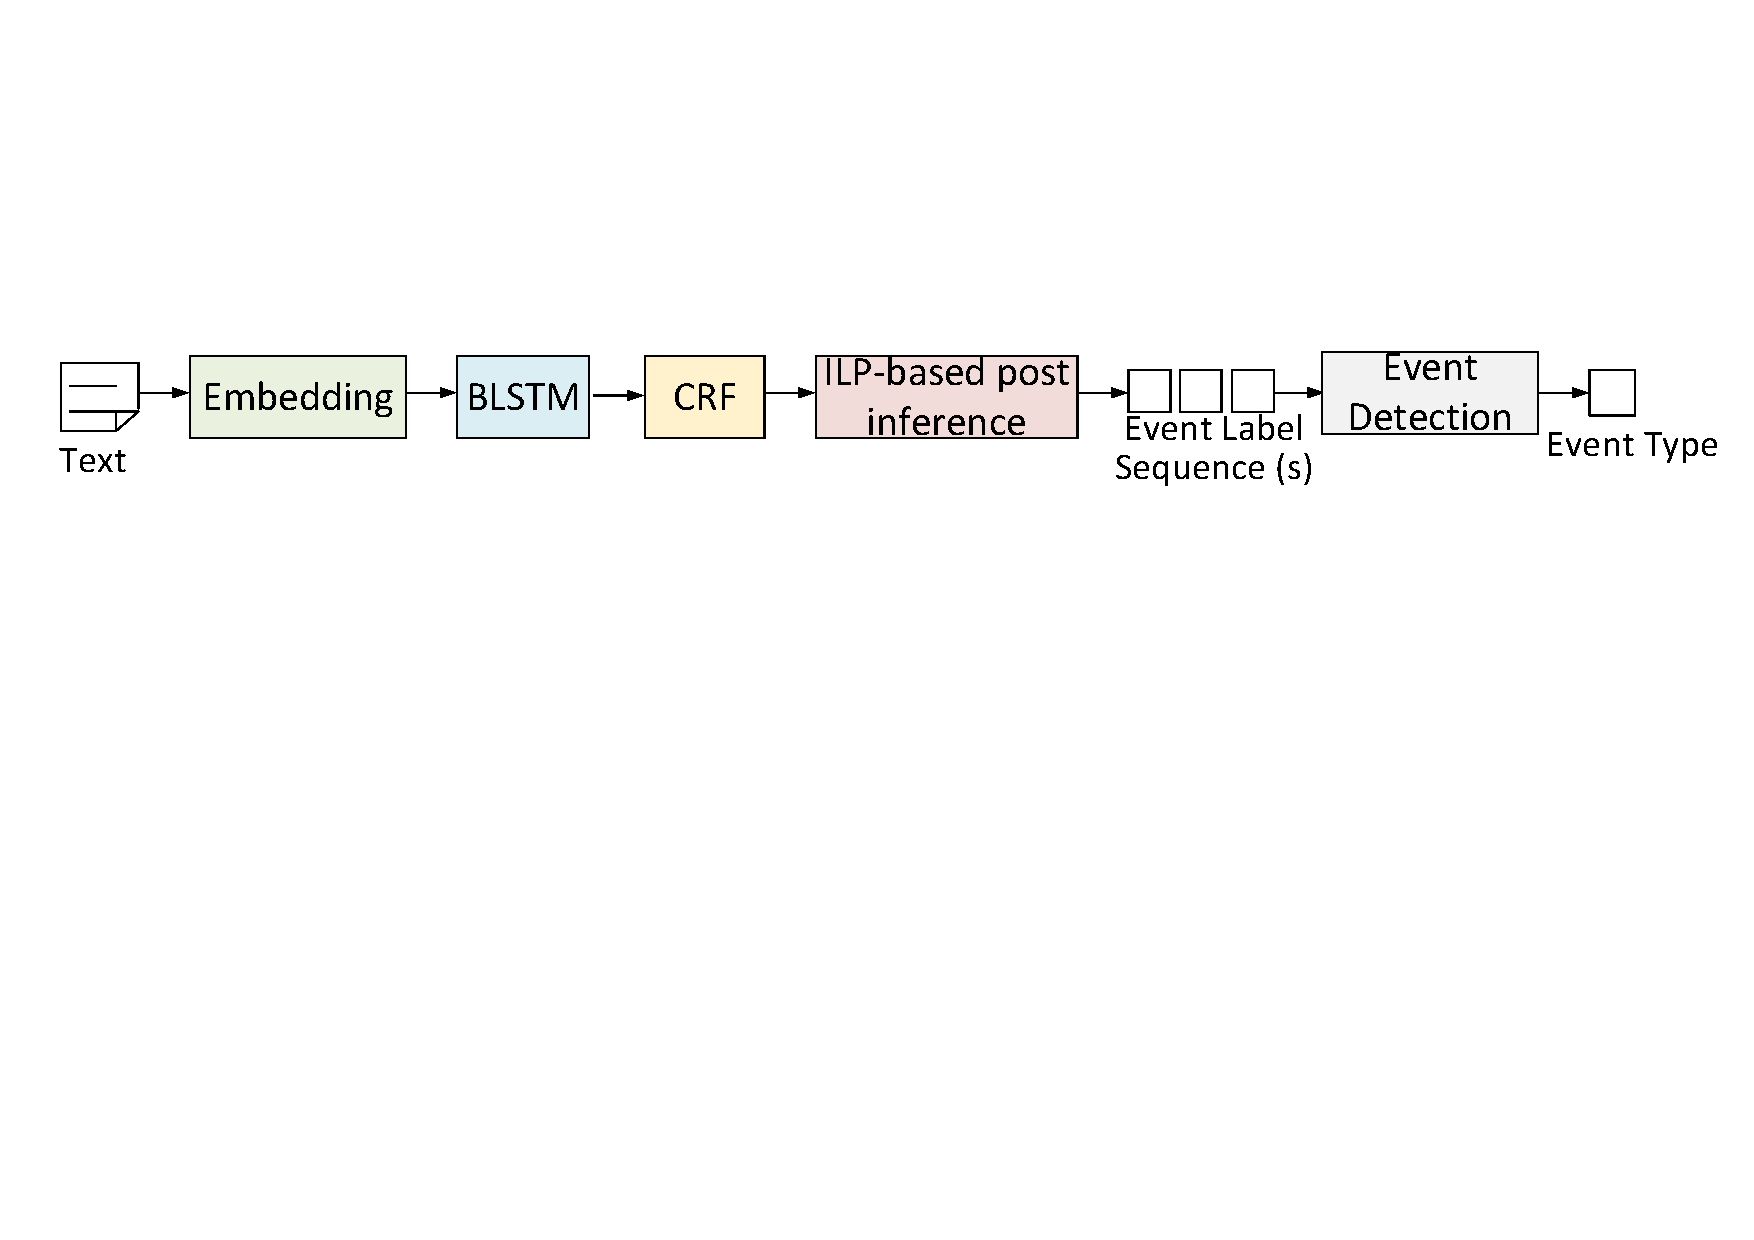
\includegraphics[width=0.5\textwidth]{figs/model.pdf}
  \caption{Our event and argument detection pipeline.}\label{fig:model}
\end{figure}

Figure~\ref{fig:model} depicts our two-stage pipeline. \FIXME{Describe the pipeline, explain the input and output of each stage.}.

\paragraph{Labeling Scheme}
Because 68\%  of  arguments in our dataset consist of more than one word, we formulate each step in a sequence labeling paradigm rather
than word-level classifications. Each word in the given sentence is tagged using the \texttt{BIO} scheme (see Figure~\ref{fig:ls}).

\subsection{Event and Key Argument Detection \label{evede}}
%Before presenting our model,
%Our event detector is an BLSTM-CRF model with ILP-based inference.
%We first present our solution for multi-words arguments, and then introduce each component in our model.
%BLSTM-CRF-ILP$_{multi}$ model, from bottom to top.

%\paragraph{Tagging scheme}

Our model for event detection has two key components, a Bidirectional LSTM (BLSTM) network with a conditional random field (CRF) layer and
an Integer Linear Programming (ILP) based post inference. The input to our model is the raw text. The BLSTM-CRF layer finds the optimal
labeling sequence which will then be post-processed by an ILP solver. It is to note that at this stage we do not concern non-key arguments
and all non-key arguments tokens will be tagged as \texttt{O}.  Using the labeling sequence, an event detector then simply maps the
sentence to a specific event type, checking if a sentence contains all the key arguments of that event type. If multiple labeling sequences
are generated, our model will map each sequence to an event type. This essentially implements a multi-typed event detection scheme.

\paragraph{BLSTM}
The Long Short-Term Memory (LSTM) network~\cite{hochreiter1997long} is a natural fit for sequence labeling, which maintains a memory based
on historical contextual information. Formally, given a sentence $\bm{w} = \{w_1, w_2, \dots, w_n\}$ of length $n$, we use $\textbf{x}_t$
to represent feature vector, e.g., word embeddings, corresponding to the $t$-th word $w_t$. At each time $t$, a forward LSTM layer takes
$\textbf{x}_t$ as input and computes the output vector $\overrightarrow{\textbf{h}}_t$ of the past context, while a backward LSTM layer
reads the same sentence in reverse and outputs $\overleftarrow{\textbf{h}}_t$ given the future context. We concatenate these two vectors to
form the output vector of a BLSTM, which is fed into a softmax layer to estimate a probability distribution over all possible labels.

\paragraph{CRF}
A straightforward way to find the label sequence for given sentence is to choose the
best label for each word individually according to the BLSTM output.
%with maximum probability by LSTM as the prediction for each word.
However, this greedy strategy ignores the dependencies between labels, thus cannot guarantee the best sequence.  %this independent labeling strategy
%is limited especially when there are strong dependencies and constraints between labels.
%To model the correlations between labels,
Therefore, we introduce a CRF layer over the BLSTM output, which is shown to be effective in various sequence labeling tasks~\cite{collobert2011natural,huang2015bidirectional}. %, such as POS tagging and NER .

We consider $\textbf{P}$ to be a matrix of confidence scores output by BLSTM, and the element $\textbf{P}_{i,j}$ of the matrix denotes the probability of the label $j$ for the $i$-th word in a sentence. The CRF layer takes a transition matrix $\textbf{A}$ as parameter, where $\textbf{A}_{i,j}$ represents the score of a transition from label $i$ to label $j$. The score of a sentence $\bm{w}$ along with a path of labels $\bm{y} = \{y_1, y_2, \ldots, y_n\}$ is measured by the sum of BLSTM outputs and transition scores:
\begin{equation}
	score(\bm{w}, \bm{y}) = \sum\limits_{i=0}^n\textbf{P}_{i, y_i} + \sum\limits_{i=1}^n\textbf{A}_{y_i, y_{i+1}},
\end{equation}
During test, given a sentence $\bm{w}$, we adopt the Viterbi algorithm~\cite{rabiner1989tutorial} to find the optimal label sequence with the maximum score among all possible label sequences.

\paragraph{ILP-based Post Inference}
Essentially, event detection is a structure prediction problem. However, the output sequences of BLSTM-CRF do not necessarily satisfy the
structural constraints. For instance, regardless of how many key arguments are correctly identified by BLSTM-CRF, if there is one key
argument missing, this detection should be considered as failed.

We thus propose to apply ILP to further globally optimize the BLSTM-CRF output  to produce the best label sequence. Formally, let
$\mathcal{L}$ be the set of possible argument labels. For each word $w_i$ in the sentence $\bm{w}$ and a pair of labels $ \langle l, l'
\rangle \in \mathcal{L} \times \mathcal{L}$, we create a binary variable ${v_{i,l,l'} \in \{0, 1\}}$, denoting whether or not the $i$-th
word $w_i$ is tagged as label $l$ and its following word $w_{i+1}$ is tagged as label $l'$ at the same time. The objective of ILP is to
maximize the overall score of the variables as:
\begin{displaymath}
	\sum\nolimits_{i, l, l'}v_{i,l,l'} * (\textbf{P}_{i,l}+\textbf{A}_{l,l'}) .
\end{displaymath}
where we consider the following four constraints:

\textbf{C1}: Each word should be and only be annotated with one label, i.e.:
\begin{equation}
	\sum\nolimits_{l,l'}v_{i,l,l'}=1
\end{equation}

\textbf{C2}: If the value of $v_{i,l,l'}$ is $1$, then there has to be a label $l^*$ that will make $v_{i+1,l',l^*}$ equal to $1$, i.e.:
\begin{equation}
	v_{i,l,l'} = \sum\nolimits_{l^*}v_{i+1,l',l^*}
\end{equation}

\textbf{C3}: If the current label is \texttt{I-arg}, then its previous label must be \texttt{B-arg} or \texttt{I-arg}, i.e.:
\begin{equation}
	v_{i,\texttt{I-arg},l'} = v_{i-1,\texttt{B-arg},\texttt{I-arg}} + v_{i-1, \texttt{I-arg}, \texttt{I-arg}}
\end{equation}

\textbf{C4}: For a specific event type, all its key arguments should co-occur in the sentence, or none of them appears in the resulting sequence. For any pair of key arguments $arg_1$ and $arg_2$ with respect to the same event type, the variables related to them are subject to:
\begin{equation}
	\sum\nolimits_{i,l'}{v_{i,\texttt{B-arg}_1,l'}} \leq n * \sum\nolimits_{j,l^*}{v_{j,\texttt{B-arg}_2,l^*}}
\end{equation}
where $n$ is the length of the sentence.

\paragraph{Multi-typed Events}
There are scenarios where one event is associated with multiple types, but all current event extractors only map a sentence to one event.
\FIXME{zw: we need an example here.} One of the advantages of our approach is that it can be easily extended to support multi-typed events.
To do so, we allow our ILP solver to output multiple optimal sequences. Specifically, after our model outputs the best sequence $\bm{s}^t$
at time $t$, we remove the previously best solutions
 $\{\bm{s}^1, \ldots, \bm{s}^{t}\}$ from the solution space, and re-run our solver to obtain the next optimal sequences $\bm{s}^{t+1}$.
We repeat the optimization procedure until the difference between the scores of $\bm{s}^1$ and $\bm{s}^T$ is greater
than a threshold $\lambda$, and consider all solutions $\{\bm{s}^1, \bm{s}^2, \ldots, \bm{s}^{T-1}\}$ as the optimal label sequences.
We use Gurobi~\cite{gurobi} as our ILP solver and set $\lambda=0.05 \times n$, which averagely produce~1.07 optimal sequences for each sentence.

\subsection{Non-key Argument Detection}
After event detection, a sentence will be classified into a or more than one event types, and labeled with its corresponding key arguments.
%The next step is argument detection, which
Next, we will identify the remaining non-key arguments in the sentence.

We adopt the same BLSTM-CRF architecture (that is used for event detection) for argument detection, where we encode the event label (output
of event detection) of each word into a key-argument feature vector through a look-up table, and concatenate it with the original word
embedding as the input to the new BLSTM-CRF. Note that we do not need post inference here, \FIXME{because...}.

\section{Experiments}
%\subsection{Experimental Setup}
%\textbf{Dataset and Evaluation Methodology}.
Our experiments are designed to answer: 1) whether it is possible to automatically collect training data for event extraction, 2) whether
extractors trained on such data can detect events of interest and identify their corresponding arguments, and 3) whether our solution can
work with other knowledge resources for more types of event.

 \subsection{Dataset Evaluation}\label{sec:evalhypo}
We start by comparing key argument selection strategies: %different data-collecting strategies:
(1) \emph{ALL}: use all arguments as key arguments; (2) \emph{IMP}:
uses the top half arguments with highest importance scores as key arguments;
%we select the top half arguments with highest importance values as key arguments;
(3) \emph{IMP\&TIME}:  includes a time-related argument together with  the arguments selected by \emph{IMP};
and (4) \emph{DIS}: eliminate sentences where the dependency distances
 between any two key arguments are greater than 2.
%(3) \emph{IMP\&TIME} means adding a time-related argument with the highest importance value to %the set of key arguments defined by
%\emph{IMP}; (4) \emph{DIS}: we eliminate sentences where the dependency distances between any two key arguments are greater than 2.
We follow the above methods to collect datasets using Freebase and the English Wikipedia dump of 2016-11-20,
randomly select 100 sentences from each dataset, and ask two annotators to decide whether each sentence implies a given type of event.



%To investigate the possibility of automatically constructing training data for event extraction,

As shown in Table~\ref{tab:3}, it is not surprising that \emph{ALL}, as the most strict, guarantees the quality of the collected data, but only contributes 203 sentences covering 9 event types, which is far from sufficient for further applications. \emph{IMP} relaxes \emph{ALL} by allowing the absence of non-key arguments, which expands the resulting dataset, but introduces more noise.
We can also see that the dependency constraint (DIS) improves the data quality (\emph{IMP}+\emph{DIS}).
%indicating that \emph{T2} is inappropriate to be used as a soft constraint.
Compared with \emph{IMP}, the significant quality improvement by \emph{IMP\&TIME} proves that time-related arguments within CVT schemas are critical to imply an event occurrence. Among all strategies, the dataset by \emph{IMP\&TIME}+\emph{DIS}  achieves the best quality, while still accounting for 46735 sentences with 50109 events, almost 10 times more than the ACE dataset, showing that it is feasible to automatically collect quality training data for event extraction without either human-designed event schemas or \textbf{extra} human annotations.
% our hypothesis \emph{H3} and \emph{H4} are feasible and it is an effective way to generate reliable data automatically.

Our final dataset, \textbf{FBWiki}, using \emph{IMP\&TIME}+\emph{DIS} , contains 46,735 positive sentences and 79,536 negative ones\footnote{Besides trivial negative samples that have no matched arguments, we randomly sample 34,837 negative instances that contain only part of key arguments, and 21,866 sentences whose key arguments violate the dependency constraint.}
 a random split of 101,019 for
training and 25,252 for testing. There are on average 4.8 arguments per event, and in total, 5.5\% instances labeled with more than two
types of events.


\begin{table}[t!]
\scriptsize
\centering
\begin{tabular}{lccc}
     \toprule
	 \textbf{Strategy} & \textbf{Sentences} & \textbf{Type} & \textbf{Positive Percentage (\%)} \\
     \midrule
	 \rowcolor{Gray}\emph{ALL} & 203 & 9 & 98\% \\
	 \emph{IMP} & 318K & 24 & 22\% \\
	 \rowcolor{Gray} \emph{IMP}+\emph{DIS} & 170K & 24 & 37\% \\
	 \emph{IMP\&TIME} & 112K & 24 & 83\% \\
	 \rowcolor{Gray} \emph{IMP\&TIME}+\emph{DIS} & 46K & 24 & 91\% \\
     \bottomrule
\end{tabular}
\vspace{-2mm}
\caption{Statistics of the datasets built with different strategies.
% \textit{Instances} denotes the number of CVT instances that can be used for each hypothesis.
%\textit{Sent.} is the number of sentences found.
\textit{Type} the number of different CVT types found.
%\textit{Positive} is the percentage of sentences mentioning the given events explicitly.
\label{tab:3}}
\vspace{-3mm}
\end{table}


%Statistics for the generated dataset from Freebase is shown in Table~\ref{statistics}.

%\begin{table}
%\small
%\centering
%\begin{tabular}{|l|c|c|c|} \hline
%& Train & Dev & Test \\ \hline
%\emph{\#PosSent.} & 29912 & 7477 & 9346 \\ \hline
%\emph{\#NegSent.} & 50904 & 12726 & 15906  \\ \hline
%\emph{\#Eve.} &  &  &  \\ \hline
%\emph{\#Arg.} &  &  &  \\ \hline
%\emph{\%Multi\_Eve.} &  &  &  \\ \hline
%\end{tabular}
%\caption{Statistics for the generated dataset. \emph{\#PosSent.} is the number of positive sentences, \emph{\#NegSent.} is the number of positive sentences, \emph{\#Eve.} is the number of event mentions, and \emph{\#Arg.} is the number of event arguments. \emph{\%Multi\_Eve.} is the ratio of multi-type events.
%, and \emph{\%Multi\_Arg.} is the ratio of multi-word arguments.
%\label{statistics}}
%\end{table}

%%%% containing 7,180 sentences, containing 7,394 events and 25,840 arguments. We then randomly select 4,800 sentences for training and 1,180 sentences as test set, and the rest 1,200 sentences for validation.
%We first manually evaluate the quality of our test set and then regard the automatically generated data as gold standard and evaluate our model accordingly. Next, we manually evaluate a subset of events detected by our model and analyze the differences with regards to the automatic evaluation. Finally, we conduct evaluation on a smaller dataset constructed according to Wikipedia tables and articles.
\vspace{2mm}

\noindent\textbf{\emph{Trigger Inference}: \mbox{ }} To further explore the relationship between key arguments and triggers, we regard the
least common ancestor of all key arguments in the dependency tree as a trigger candidate. As listed in Table~\ref{freqTriggers}, these
candidates share similar meanings and are highly informative to the underlying event types, showing that our key arguments with necessary
constraints can play the same role with explicit triggers in identifying an event.
% Although missing explicit information from \KB, most triggers can be inferred from the dependencies between a group of key arguments and its context.

\begin{table}
	\scriptsize
	\centering
	\begin{tabular}{lll}
    \toprule
		\textbf{Event types} & \textbf{Trigger candidates} & \textbf{Percentage} \\
    \midrule
		\rowcolor{Gray}film\_performance & play, appear, star, cast, portray & 0.72 \\
		award\_honor & win, receive, award, share, earn & 0.91 \\
		\rowcolor{Gray}education & graduate, receive, attend, obtain, study & 0.83 \\
		acquisition & acquire, purchase, buy, merge, sell & 0.81 \\
		\rowcolor{Gray}employ.tenure & be, join, become, serve, appoint & 0.79 \\
    \bottomrule
	\end{tabular}
    \vspace{-2mm}
	\caption{Top 5 most frequent trigger candidates and their proportions over all positive instances within each type.}
    \vspace{-3mm}
	\label{freqTriggers}
\end{table}

\vspace{2mm} \noindent\textbf{\emph{On ACE}: \mbox{ }} We also test our strategy on the ACE dataset. We first collect all annotated events,
without triggers, as the knowledge base to compute the importance values for all arguments, and select the key arguments for each ACE event
type accordingly. We follow \emph{IMP\&TIME}+\emph{DIS} to examine every sentence whether it can be selected as an annotated instance
within the ACE event types. Eventually, we correctly obtain 3,448 sentences as positive instances, covering 64.7\% of the original ACE
dataset.  We find that the main reason for the missing 35.3\% is that many arguments in the ACE dataset are pronouns, where our strategy is
currently unable to treat pronouns as key arguments. However, if a high-precision coreference resolution tool is available to preprocess
the document,
our solution would be able to automatically label more instances.% as training data.
% \textbf{ANYTHING NOVEL that traditional ACE does not have??? multple types? multiple events?}

 \subsection{Extraction Setup}\label{sec:evalevent}
Next, we evaluate our event extractor on FBWiki  %the collected datasets,
%\paragraph{Metrics:} We evaluate our models
%in terms of popular metrics in event extraction, i.e.,
with \emph{precision} (P), \emph{recall} (R), and \emph{F-measure} (F) for each subtask. These metrics are computed according to the
following standards of correctness. For \emph{event classification}, an event is correctly classified if its reference sentence contains
\textbf{all key arguments} of this event type. For \emph{key argument detection}, an event is correctly detected if its type and all of its
key arguments match a reference event within the same sentence. For \emph{all argument detection}, an event is correctly extracted if its
type and all of its arguments match a reference event within the same sentence.

\vspace{2mm}


\noindent \textbf{\emph{Training}:} All hyper-parameters are tuned on a development split in the training set. During event detection, we
set the size of word embeddings to 200, the size of LSTM layer to 100. In argument detection, we use the same size of word embedding, while
the size of LSTM layer is 150, and the size of key argument embedding is 50. Word embeddings are pre-trained using skip-gram
word2vec~\cite{mikolov2013distributed} on English Wikipedia and fine tuned during training. We apply dropout (0.5) on both input and output
layers.




\vspace{2mm}\noindent\textbf{\emph{Baselines}:}
%To investigate the effectiveness of our proposed model,
We compare our proposed model with three baselines.
The first is a  BLSTM model that takes word embeddings as input, and outputs the label for each word with the maximum probability. % among all possible labels.
For feature-based methods, we apply CRF (using the CRF++ toolkit~\cite{kudo2005crf++} ) and Maximum Entropy \cite{berger1996maximum} (Le
Zhang's MaxEnt toolkit) to explore a variety of elaborate features, according to the state-of-art feature-based ACE event
extractors~\cite{li2013joint}. Note that after key argument detection, we add the resulting label of each word as a supplementary feature
to detect non-key arguments.

\subsection{Compare with Automatic Annotations}
Firstly, we compare the model output against the automatically obtained event annotations.
As shown in Table~\ref{tab:1}, feature-based models perform worst in both event classification and argument detection.
One of the main reasons is the absence of explicit trigger annotations in our dataset, which makes it impossible to include trigger-related features, e.g., trigger-related dependency and position features.
Although traditional models can achieve higher precisions, they only identify a limited number of events, resulting in low recalls.
Neural-network methods perform much better than feature-based models, especially in recall, since they can make better use of word semantic features. Specifically, BLSTM can capture longer dependencies and richer contextual information, instead of neighbouring word features only.
The CRF layer brings an averagely 2\% improvement in all metrics, and by adding the ILP-based post inference, our full model, BLSTM-CRF-ILP$_{multi}$, achieves the best performance among all models.
% Moreover, neural-network-based methods can avoid errors propagating from other NLP preprocessing tools like POS tagging and NER.

\begin{table*}[!t]
\centering
\scriptsize
\begin{tabular}{|l|p{1.cm}<{\centering}|p{1.cm}<{\centering}|p{1.cm}<{\centering}|p{1.cm}<{\centering}|p{1.cm}<{\centering}|p{1.cm}<{\centering}|p{1.cm}<{\centering}|p{1.cm}<{\centering}|p{1.cm}<{\centering}|} \hline
	\multirow{2}{*}{\textbf{Model}} & \multicolumn{3}{c|}{\textbf{Event Type}} & \multicolumn{3}{c|}{\textbf{Key Argument Detection}} &
	\multicolumn{3}{c|}{\textbf{All Argument Detection}} \\ \cline{2-10}
	 & \textbf{P} & \textbf{R} & \textbf{F} & \textbf{P} & \textbf{R} & \textbf{F} & \textbf{P} & \textbf{R} & \textbf{F }\\ \hline
	\rowcolor{Gray} CRF & 88.9 & 11.0 & 19.6 & 36.1 & 4.47 & 7.96 & 19.9 & 3.06 & 5.30  \\ \hline
	MaxEnt & \textbf{95.2} & 12.4 & 21.9 & 41.6 & 5.40 & 9.56 & 22.5 & 3.40 & 5.91 \\ \hline
	\rowcolor{Gray} BLSTM & 89.8 & 63.0 & 74.1 & \textbf{64.9} & 45.5 & 53.5 & 42.9 & 27.7 & 33.7  \\ \hline \hline
	BLSTM-CRF & 86.4 & 67.4 & 75.7 & 63.6 & 49.6 & 55.8 & \textbf{44.4} & 31.0 & 36.5  \\ \hline
	\rowcolor{Gray} BLSTM-CRF-ILP$_{1}$ & 84.4 & 74.1 & 78.9 & 62.3 & 53.8 & 57.3 & 42.7 & 33.8 & 37.7 \\ \hline
	BLSTM-CRF-ILP$_{multi}$ & 85.3 & \textbf{79.9} & \textbf{82.5} & 60.4 & \textbf{55.3} & \textbf{57.7} & 41.9 & \textbf{34.6} & \textbf{37.9} \\ \hline
\end{tabular}
\caption{System performance when compared against automatic annotations (\%).  \label{tab:1}}
\end{table*}

% \paragraph{Multi-word Argument Detection}
% Committing to the multi-word argument issue, we treat each subtask as a sequence labeling problem. Evaluated on multi-word arguments, the F1 scores of BLSTM-CRF, BLSTM-CRF-ILP$_1$ and BLSTM-CRF-ILP$_{multi}$ in argument detection are 71.3\%, 80.5\%, and 81.0\%, respectively.

%\paragraph{The CRF Layer:}
%As seen in Table~\ref{tab:1},
It is not surprising that  every model with a CRF layer over its BLSTM layer is superior to the one with a BLSTM layer only. Compared with vanilla BLSTM, BLSTM-CRF achieves higher precisions and recalls in all subtasks by significantly reducing the invalid labelling sequences (e.g., \texttt{I-arg} appears right after \texttt{O}). During prediction, instead of tagging each token independently, BLSTM-CRF takes into account the constraints between neighbouring labels, and potentially increases the co-occurrences of key arguments regarding the same event type. % in some way.

%\paragraph{The ILP Post Inference:}
As shown in Table~\ref{tab:1}, the ILP-based post inference considerably improves the overall performance, especially in \textit{event type classification}. With the help of constraint \textbf{C4},  dubious key arguments can be correctly inferred through other key arguments from their context. Compared with BLSTM-CRF, BLSTM-CRF-ILP$_1$ produces an F1 gain of 3.2\% in event type classification, 1.5\% in key argument detection, and 1.2\% in all argument detection. %, with respect to tF1.

\vspace{2mm}\noindent\textbf{\emph{Multi-type Events}:}
%We further investigate the effect of
Among all methods, BLSTM-CRF-ILP$_{multi}$ is the only model that can deal with multi-type event mentions. %As shown in Table~\ref{tab:1},
The proposed strategy ILP$_{multi}$ helps detect more event mentions for a sentence, contributing to the increase of recalls, and F1 scores with a little drop of precisions.
%\textbf{Evaluated on \textbf{38XXXX} sentences containing multi-type event mentions, the F1 scores of BLSTM-CRF-ILP$_{multi}$ in event type classification, event detection and argument detection are 70.7\%, 58.4\% and 26.9\%, respectively.}
BLSTM-CRF-ILP$_{multi}$ can correctly identify 132 sentences with multi-type events,
with an accuracy of 95.6\%, and for each involved event, our model maintains a high
performance in identifying its arguments, achieving 45.5\%, and 29.1\% in F1 for key argument detection and all argument detection, respectively.

\subsection{Manual Evaluation}\label{manualeve}
To provide a deep investigation about our dataset and models, we randomly sample 150 sentences
from the test set. Two annotators are asked to annotate each sentence following
two steps. First, determine whether a given sentence is positive or negative, and assign \textbf{all possible}
event types to positive ones. Next, label all related arguments and their roles according to
the event types for all positive instances. Two annotators will independently annotate each sentence,
and discuss to reach an agreement. The inter-annotator agreement is 87\% for event types and 79\% for arguments.


By comparing the automatic and manual annotations on the 150 sentences, we find that
the main issue for the automatic annotation is that some automatically labeled sentences
do not imply any event while still matching all key properties of certain CVT entries in Freebase.
We find 16 such instances that are mistakenly labeled as positive.
For example in Figure~\ref{fig:1}, although the phrase \underline{\emph{the car}} in S6 matches a film name,
it does not indicate that film. %, and there is no explicit evidence indicating that an actor starred in this film.
This is mainly because that we currently do not have a strong entity linker to verify those entities, which we leave for
future work.
But, interestingly,
% a bottleneck of our data generation strategy.
during manual investigation,
%we find 16 negative sentences which are mistakenly labeled as positive, and
we find that BLSTM-CRF-ILP$_{multi}$ manages to detect 6 of them as negative.


%\begin{table}[h]
%\scriptsize
%\centering
%\begin{tabular}{|l|p{0.8cm}<{\centering}|p{0.8cm}<{\centering}|p{0.8cm}<{\centering}|} \hline
%	% Model & EC & AD & ED \\ \hline
%	% CRF & 21.2 & 13.3 & 5.30 \\ \hline
%	% MaxEnt & 17.7 & 11.7 & 5.44 \\ \hline
%	% BLSTM & 79.8 & 64.3 & 41.2 \\ \hline \hline
%	Model & EC & KAD & AAD \\ \hline
%	BLSTM-CRF & 75.4 & 54.7 & 35.5 \\ \hline
%	BLSTM-CRF-ILP$_{1}$ & 77.2 & 56.1 & 35.7 \\ \hline
%	BLSTM-CRF-ILP$_{multi}$ & \textbf{80.7} & \textbf{56.4} & \textbf{36.3} \\ \hline
%\end{tabular}
%\caption{The F1 scores of different systems on the manually annotated data. EC, KAD, AAD denote the event type classification, key argument detection and all key argument detection, respectively. \label{tab:2}}
%\end{table}

On this manually annotated dataset, we can observe similar trends with Table~\ref{tab:1}, and BLSTM-CRF-ILP$_{multi}$ remains the best performing model, achieving 80.7\%, 56.4\% and 36.3\% in F1 scores for event type, key argument detection and all argument detection, respectively.
%where we can observe similar trends with Table~\ref{tab:1}, that
%both CRF layer and ILP$_{multi}$ greatly improve the overall performance and

%Table~\ref{tab:2} summarizes the performances of different models on the manually annotated dataset, where we can observe similar trends with Table~\ref{tab:1}, that
%both CRF layer and ILP$_{multi}$ greatly improve the overall performance and
% shows the system performances in the manual evaluation. We can draw similar conclusions about the comparison of performances between different models as automatic evaluation. It is clear that
%BLSTM-CRF-ILP$_{multi}$ remains the most effective model. %,  in event extraction as it achieves the highest F1 scores in both manual and automatic evaluation.

\begin{figure}[t!]
	\centering
	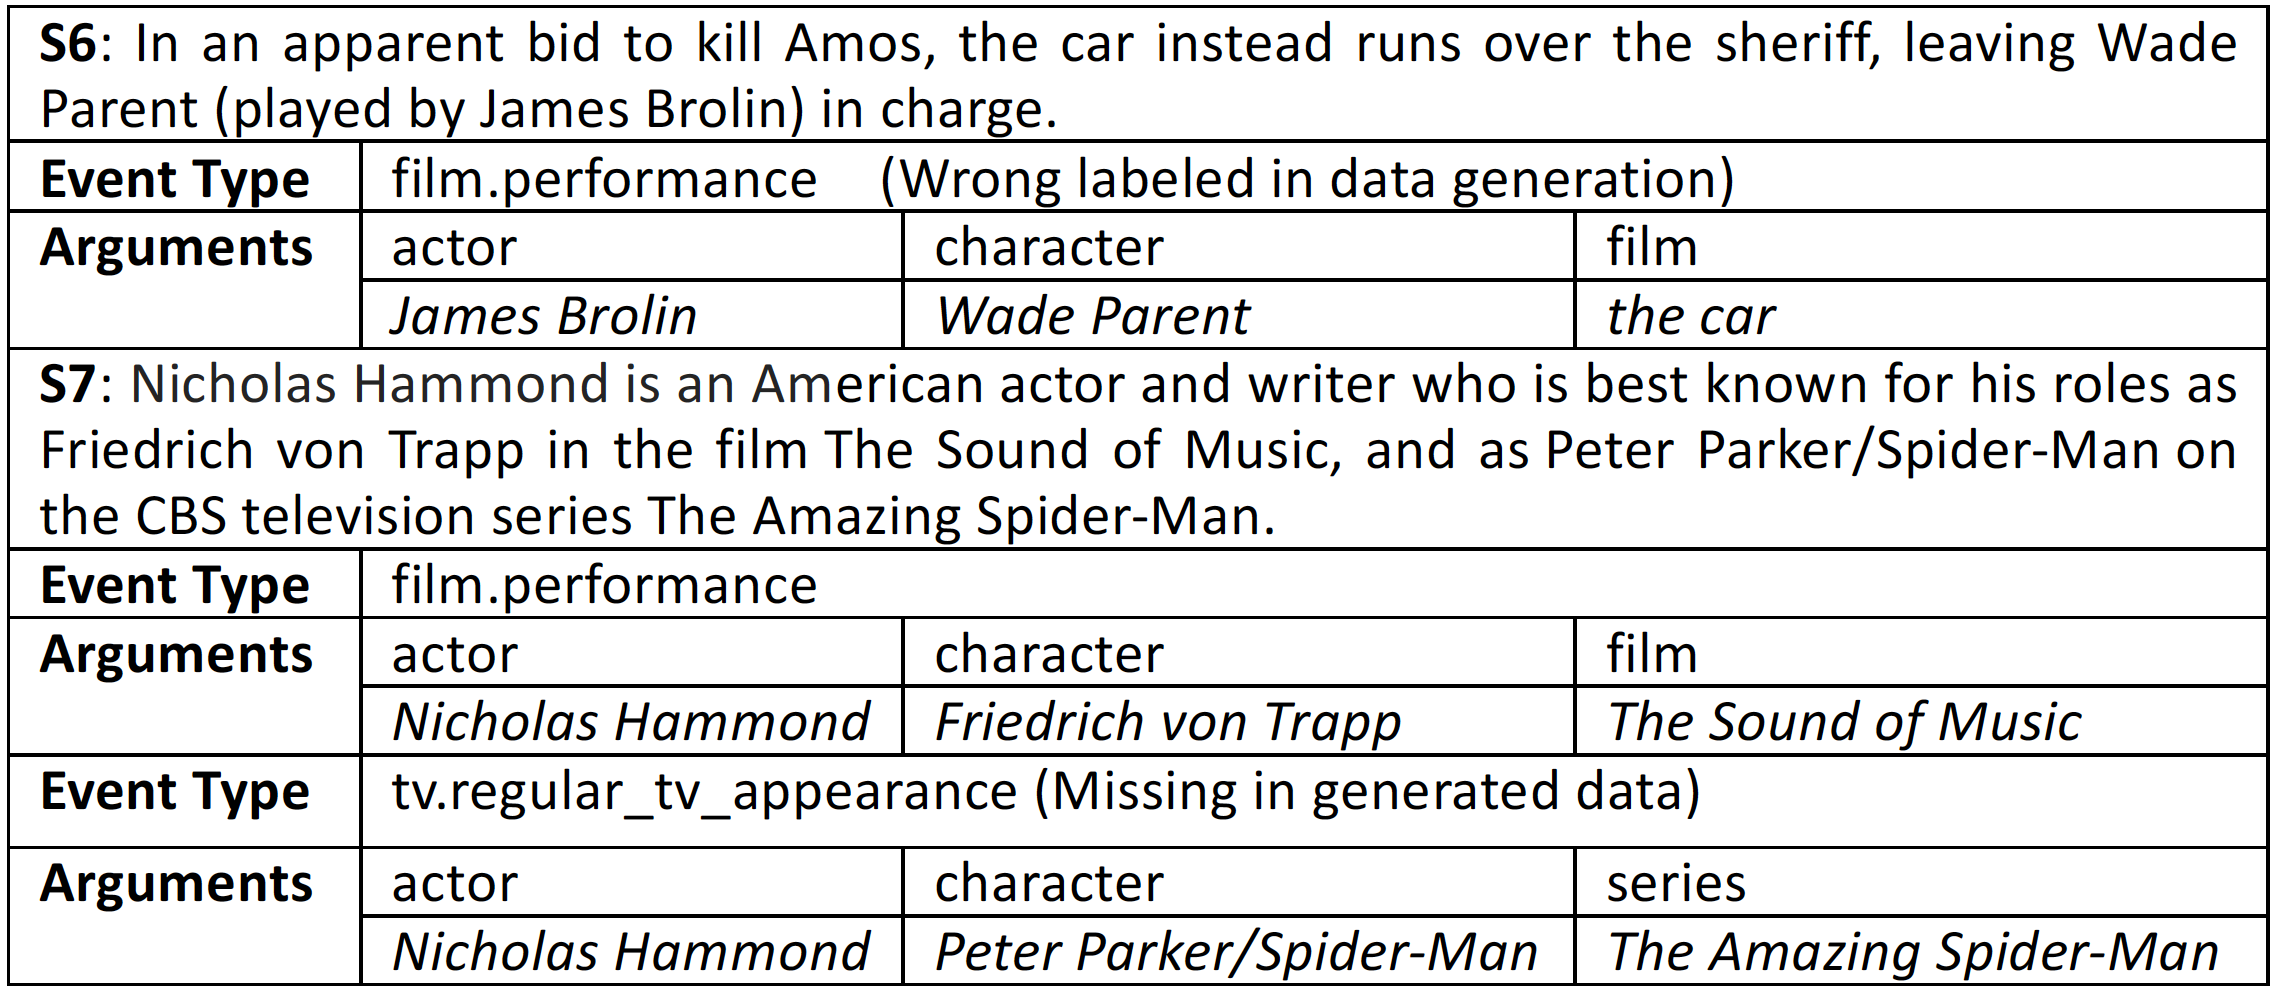
\includegraphics[width=.48\textwidth]{figure3(3).png}
    \vspace{-3mm}
	\caption{Example outputs of BLSTM-CRF-ILP$_{multi}$.\label{fig:1}}
    \vspace{-3mm}
\end{figure}



%Moreover, %manual evaluation may help us to gain a deep insight about our data and models. We
% we manually check the top 5 event types whose EC F1 scores by BLSTM-CRF-ILP$_{multi}$ differ greatly between automatic evaluation and manual evaluation, summarized in Table~\ref{tab:4}. We find that most of the performance differences are caused by data generation. Figure~\ref{fig:1} examples two types of errors in data construction. Several automatically labeled sentences do not imply any event while still matching all key properties of some CVT entries. For example, although the phrase \emph{the car} in S5 matches a film name, it does not indicate this film, and there is no explicit evidence indicating that an actor starred in this film. This is a bottleneck of our data generation strategy. During manual evaluation, we find 16 negative sentences which are mistakenly labeled as positive, and our model manages to rectify 6 of them.

Remarkably, our BLSTM-CRF-ILP$_{multi}$ model can find more \CVT instances that are currently not referenced in Freebase. Our model detects two events in S7, while the arguments of the \textit{tv.tv\_appearance} event do not match any existing CVT instances in Freebase, which do not receive any credit during automatic evaluation, but should be populated into Freebase. %leading to a missing event in data generation.
This  suggests that by learning from distant supervision provided by Freebase, our model can be used to populate or update Freebase instances in return.

%\begin{table}[h]
%\small
%\centering
%\begin{tabular}{|l|c|c|c|} \hline
%	Event type & P & R & F \\ \hline
%	olympics.medal\_honor%\footnote{The full name is olympics.olympic\_medal\_honor in Freebase.}
%	& $\downarrow$ 25.0\% & $\downarrow$ 5.0\% & $\downarrow$ 13.8\% \\ \hline
%	film.performance & $\downarrow$ 21.4\% & $\uparrow$ 3.1\% & $\downarrow$10.3\% \\ \hline
%	business.acquisition & $\rightarrow$ & $\downarrow$ 7.1\% & $\downarrow$ 5.4\% \\ \hline
%	tv.appearance%\footnote{The full name is tv.regular\_tv\_appearance in Freebase.}
%	& $\downarrow$ 9.5\% & $\uparrow$ 3.0\% & $\downarrow$ 3.1\% \\ \hline
%	film.release%\footnote{The full name is film.film\_regional\_release\_date in Freebase.}
%	& $\downarrow$ 7.7\% & $\uparrow$ 5.6\% & $\downarrow$ 0.55\% \\ \hline
%\end{tabular}
%\caption{The difference of EC F1 scores (by BLSTM-CRF-ILP$_{multi}$) between automatic and manual evaluation for top 5 event types.\label{tab:4}}
%\end{table}

\vspace{2mm}\noindent\textbf{\emph{On BBC News}:}
% 在BBC新闻上抽取business.acquisition和tv.regular_tv_appearance两类事件,并用规则更新
We further apply our event extractor, trained on FBWiki, to 397 BBC News
articles (2017/04/18 -- 2017/05/18 in Politics, Business and TV sections), and manually examine the extraction results. We find that our model is able to correctly identify 117 events, and 53 events,
almost half of which are not covered in the currently used Freebase.



\subsection{Tables as Indirect Supervision}
To investigate the applicability of our approach to other structured knowledge/tables besides Freebase \CVT tables, we automatically build
a new dataset, \textbf{TBWiki}, with the supervision provided by Wikipedia tables, which characterize events about business acquisition,
winning of the Olympics games, and awards winning in entertainment (Table~\ref{tab:6}).

\begin{table}[t]
\scriptsize
\centering
\begin{tabular}{lccccc}
    \toprule
	\textbf{Event type} & \textbf{Entries} & \textbf{Positive} & \textbf{EC} & \textbf{KAD} & \textbf{AAD} \\
    \midrule
	\rowcolor{Gray} Acquisition & 690 & 414 & 87.0\% & 72.0\% & 69.6\% \\
	Olympics & 2503 & 1460 & 77.2\% & 64.5\% & 38.6\% \\
	\rowcolor{Gray} Awards & 3039 & 2217 & 95.0\% & 82.8\% & 58.6\% \\
    \bottomrule
\end{tabular}
\caption{Statistics of the TBWiki dataset and the performance (in F1) of our model on TBWiki.
%\textit{Entr.} is the number of table entries. \textit{Sent.} is number of positive instances.
EC, KAD and AAD denote event type classification, key argument detection and all key argument detection, respectively.
\label{tab:6}}
\end{table}

We train our BLSTM-CRF-ILP$_{multi}$ on this dataset and evaluate it on 100 manually annotated sentences.
% and follow the same steps of event annotations as mentioned in Section~\ref{manualeve}.
We can see that without extra human annotations, %Table~\ref{tab:6} demonstrates that tabular data as distant supervision can be adapted to extract high-confidence events
our model can learn to extract events from the training data weakly supervised by Wikipedia tables. Given a specific event type, as long as we can acquire tables implying events of such type, it is possible to automatically collect training data from such tables, and learn to extract structured event representations of that type. % an effective but robust event extractor. , which is much easier than human annotation and unlimited in event types.

\section{Related Work}
%Event extraction is one of the fundamental tasks in information extraction. % and natural language understanding. 
Most event extraction works are within the tasks defined by several evaluation frameworks (e.g., MUC~\cite{grishman1996message}, 
ACE~\cite{doddington2004automatic}, ERE~\cite{song2015light} and TAC-KBP~\cite{mitamura2015event}), 
all of which can be considered as a template-filling-based extraction task.
These frameworks focus on limited number of event types, which are designed and annotated by human experts and
hard to generalize to other domains.  
%Most approaches within  these frameworks 
Furthermore, existing extraction systems, which usually adopt a supervised learning paradigm, 
have to rely on those high-quality training data within those frameworks, 
thus hard to move to more domains in practice, regardless of feature-based~\cite{gupta2009predicting,hong2011using,li2013joint} or neural-network-based methods~\cite{chen2015event,nguyen2016joint}.

Besides the works focusing on small human-labeled corpus, 
Huang et al. \shortcite{huang2016liberal} leverage various linguistic resources (e.g., FrameNet, PropBank and VerbNet) to propose a novel Liberal Event Extraction paradigm 
which automatically discovers event schemas and extract events simultaneously from any unlabeled corpus. 
In contrast, we propose to exploit existing structured knowledge bases, e.g., Freebase, to automatically discover 
types of events as well as their corresponding argument settings, without expert annotation, and further automatically
construct training data, with the essence of \DS.
 
Distant supervision~(\DS) has been widely used in binary relation extraction, where the key assumption is that 
 sentences containing both the subject and object of a $<$$subj$, $rel$, $obj$$>$ triple can be seen as its support, and further
used to train a classifier to identify the relation $rel$. However,  this assumption does not fit to our event extraction scenario, 
where an event usually involves several arguments and it is hard to collect enough training sentences with all arguments appearing in, as indicated by the low coverage of \textit{ALL}. We therefore investigate different generation strategies for event extraction within the \texttt{DS} paradigm and propose to utilize time and syntactic clues to refine the \DS assumption for better data quality. We further relieve the reliance on event trigger annotations by previous event extractors, and define a novel event extraction paradigm with key arguments to characterize an event type. 

%
%However, these the reliance on high-quality training data are usually  human-annotated, and  training data prevents  
%
%We typically divide them into feature-based methods and neural-network-based methods. 
%
%Most traditional feature-based methods %usually rely on a variety of elaborate features. They 
% aim to exploit different feature extraction strategies and evaluate their contributions. 
%Besides training classifiers for each subtask, there are also works  jointly learning trigger labeling 
%and argument labeling using structured prediction models to capture both local and global 
%features of triggers and arguments~\cite{li2013joint}. 
%
%Neural-network-based methods are free of hard feature engineering and error propagation from  external NLP tools. 
%In the neural-network side, both convolutional neural network (CNN)~\cite{chen2015event}  and RNN have been employed 
%to extract features of different levels. 
%avoid hard feature engineering and error propagation from  external NLP tools. 
%Two types of neural works have been employed. Chen et al. \shortcite{chen2015event} 
%propose a convolutional neural network (CNN) with a dynamic multi-pooling layer to capture sentence-level features better. 
%Nguyen et al. \shortcite{nguyen2016joint} benefit from  a bidirectional RNN with various memory 
%matrices to jointly learn triggers and arguments within the ACE framework.% which benefits from both joint models and neural network  models. 
%However, to our knowledge, LSTM-CRF models have not been applied in earlier studies.
%
%In contrast to these prior systems focused on small human-labeled corpus, Huang et al. \shortcite{huang2016liberal} 
%propose a novel Liberal Event Extraction paradigm which automatically discovers event schemas and extract events 
%simultaneously from any unlabeled corpus. 

\section{Conclusions}
This paper has presented a novel, fast approach to automatically construct training data for event extraction with little human
involvement, which in turn allows effective event extraction modeling. To generate training data, our approach first extracts, from
existing structured knowledge bases, which of the arguments best describe an event; then, it uses the key arguments to automatically infer
the occurrence of an event without explicit trigger identification. To perform event extraction, we develop a novel architecture based on
neural networks and post inference, which does not require explicit trigger information. We apply our approach to label Wikipedia articles
using knowledge extracted from various knowledge bases. We show that the quality of the automatically generated training data is comparable
to those that were manually labeled by human experts. We demonstrate that this large volume of high-quality training data, combining with
 our novel event extraction architecture, not only leads to a highly effective event extractor, but also enables multiple typed event
detection for the first time.




%In this paper, we propose a novel event extraction paradigm without expert-designed event templates by leveraging structured knowledge bases or tables to automatically acquire event schema and corresponding training data. We propose a BLSTM-CRF model with ILP-based post inference to extract multi-typed event mentions without explicit trigger annotations. Experimental results on both manual and automatic evaluations show that it is possible to learn to identify both typed events and typed roles with indirect supervision from Freebase or Wikipedia tables.
%In the future, we will first further investigate how to better characterize key arguments for a certain event type, and extend our work to update a structured knowledge base according to news events.
%
%%Furthermore, our model can extract information not covered by Freebase which indicates the possibility to extend this work to knowledge base population.

% \section{ Acknowledgments}

% References and End of Paper
% These lines must be placed at the end of your paper
\bibliography{aaai}
\bibliographystyle{aaai}
\end{document}
